\documentclass[11pt, journal, a4paper]{IEEEtran}

\usepackage{graphicx}   
\usepackage{url}        
\usepackage{amssymb}
\usepackage{amsmath}    
% \usepackage[backend=bibtex]{biblatex}
% Some useful/example abbreviations for writing math
% \newcommand{\argmax}{\operatornamewithlimits{argmax}}
% \newcommand{\argmin}{\operatornamewithlimits{argmin}}
% \newcommand{\x}{\mathbf{x}}
% \newcommand{\y}{\mathbf{y}}
% \newcommand{\ypred}{\mathbf{\hat y}}
% \newcommand{\yp}{{\hat y}}

\begin{document}

% Define document title, do NOT write author names for the initial submission
% \font\myfont=cmr12 at 20pt

% \title{\vspace{-1.0cm}{\myfont Quantitative Volumetric Analysis and Prediction Modeling of Hematoma Expansion in Patients with Intracerebral Hemorrhage}}
\title{Quantitative Volumetric Analysis and Prediction Modeling of Hematoma Expansion in Patients with Intracerebral Hemorrhage}
\author{Lisa Guo, Jean Law, Jun Won Park}
\maketitle

% Write abstract here
% \begin{abstract}
% 	This is a rough guide to producing the project report. 
% 	The structure outlined here is a suggestion, but you must use this template\footnote{There are also Word templates for this format (\url{https://www.ieee.org/conferences/publishing/templates.html}) if you wish; but don't forget you will submit a pdf} (of course, replace these hints/instructions/examples with your own text); a limit of 5 pages \emph{not including} references and an optional appendix. 
% 	Hint: shared tools like \texttt{http://overleaf.com/} are great for collaborating on a multi-author report in \LaTeX. 
% \end{abstract}

% Each section begins with a \section{title} command

\section{Background}
\label{sec:background}
% What is the cause of the problem?
% What is the problem?
Intracerebral Hemorrhage (ICH) refers to a medical condition caused by the tearing of a cerebral vessel, a blood vessel that supplies the brain with blood \cite{puy2023intracerebral}. This tearing allows blood to enter the brain tissue and the bleeding may collect and form a clot of blood called a hematoma \cite{hematoma}. As the hemorrhage progresses, more blood clots may form within the brain tissue, causing the hematoma to expand. 

Hematoma expansion affects approximately 20-40\% of patients with Intracerebral Hemorrhage (ICH), and research has shown that hematoma expansion serves as an important predictor of poor prognosis \cite{chen2017predictors},\cite{li2020hematoma}. Large volumes of hematoma expansions are associated with worse treatment outcomes and are shown to have increased mortality and disability \cite{dowlatshahi2011defining}. 
As a consequence, assessing hematoma volume (HV) remains a vital task for clinicians as clinicians can use this information to identify patients at high risk and determine appropriate treatment strategies to improve treatment outcomes \cite{haupenthal2023hematoma}. 

Several studies and deep learning models have been developed to segment hematoma from Computed Tomography (CT) scans. However, to the best of our knowledge, there is no open-source segmentation deep learning model specifically trained on Magnetic Resonance Imaging (MRI) scans as direct input. Consequently, clinicians who only have MRI scans of a patient would need to convert an MRI scan to a CT scan first to use the open-source segmentation models. Our team aims to develop a robust and accurate deep learning model for the segmentation of hematoma expansion from MRI scans of patients with intracerebral hemorrhage and predict the volume of hematoma expansion. 

% Introduction to our project
The imaging modality we are using is Magnetic Resonance Imaging (MRI) which is superior to other imaging modalities like Computed Tomography (CT) in terms of its capability to provide a better soft tissue contrast \cite{CenterforDevicesandRadiologicalHealth}. We can obtain a cleaner boundary between fat, fluid, muscle, and soft tissue which allows us to obtain a more accurate masking of hematoma expansion.

Note that our group does not have access to the MRI scans of the hematoma dataset yet. Hence, we will be applying our approaches to segment brain tumors from MRI scans using the BraTS dataset, provided by the organizers of the Brain Tumor Segmentation (BraTS) challenge to first test whether our approaches deserve further exploration. 

The BraTS dataset contains 2,000 Multiparametric Magnetic Resonance Imaging (mpMRI) scans of patients with brain tumors, and each scan is accompanied by masks, which essentially label information to indicate whether a given area, like a pixel of an image, is a target of interest. We can use this data to train a deep-learning model to segment brain tumors from MRI scans. 

Additionally, we are also interested in predicting HV. One way to measure HV is through the use of the 'Tada formula' which was developed specifically to calculate the volume of hematoma \cite{sha2023improvements}. We can extract the HV data from the masking data (y), the true volume of hematoma expansion, and the volume of the segmented output (x) then perform a regression task to predict the true HV. The equivalent task for this regression problem using the BraTs dataset would be to predict the volume of brain tumors.

Unlike the BraTs dataset, an evident challenge we anticipate is the lack of scans. The occurrence of ICH is approximately 25 cases per 100,000 individuals \cite{faghih2021mortality}. Moreover, within this population, only 20-40\% experience hematoma expansion \cite{haupenthal2023hematoma}. Additionally, MRI scans are expensive and not as convenient as CT scans. Thus, we anticipate difficulty in obtaining a substantial quantity of MRI scans from ICH patients with hematoma expansion to train a deep learning model from scratch. Due to the potentially limited dataset, the model trained from using this dataset may not be able to generalize well. Thus, instead of training a deep learning model from scratch, it may be better to use a pre-trained model and fine-tune the model with our dataset. 

% Result/Goal and their effects/next steps
Clinicians will be able to use our model to segment hematoma expansion. One important application is mock surgery. Clinicians can then use the segmented output to create a 3D-printed model of the hematoma and perform mock surgery before the actual operation, which will improve the operation's success rate. Clinicians can also use the predicted volume of hematoma expansion to determine the appropriate treatment strategy. We hope that our study can reduce mortality and disability among ICH patients with hematoma expansion and improve treatment outcomes.

% talk about the difficulty in obtaining MRI scans, cost, etc.
% dataset intro/ general summary of the datasets 
% # of ct scans, possibly talk about metadata?

% ct is cheap, and fast
% goal, use cases, why is it important
% segmenting (predicting volume of) hematoma expansion is critical to the diagnosis/treatment
% Hematoma expansion occurs in 20-40% of ICH cases and is a major predictor of poorer patient outcomes 
% By identifying patients at high risk, doctors can tailor treatment strategies more effectivel=

% challenges 


% Here, tell the reader everything they need to know to understand your work, in your own words. It should be written in the sense of ``it is clear \textit{you understand something when you can explain something simply, and in a way different from how you learned it}''. So this section should be pedagogical. Aim to explain concepts simply. The goal is to inform, not to impress. 

\section{Previous work review}
\subsection{Segmentation}
The manual delineation of hemorrhages by experts with radiologic image experience was traditionally seen as the gold standard for segmenting ICH from an image, but this method is time-consuming and not scalable to a large number of images. This is why machine learning methods for ICH segmentation have been extensively studied. Initially, the fuzzy clustering method (also known as soft k-means), in which images are classified into a predefined number of clusters \cite{fuzzy_cluster} was the most important clustering method for ICH segmentation. The random forest algorithm was also successfully used by Muschelli et. al in 2017~\cite{pitchperfect}: their tool ichseg first preprocesses the data, including skull stripping, before segmenting ICH from the image using random forest.

It appears that deep learning based approaches to hematoma volume (HV) prediction started to be more frequently researched into from 2019 onwards. However, these models were unable to perform well across different datasets, even on the same HV prediction task. It was hence important to develop a robust segmentation method that could reliably achieve good accuracy across different datasets. 

In the paper A Robust Deep Learning Segmentation Method for Hematoma Volumetric Detection in Intracerebral Hemorrhage~\cite{robust_dl_segmentation} published in 2022, Yu et. al developed a robust deep learning segmentation method for quick and accurate HV analysis using computed tomography. Their segmentation model, dimension reduction U-Net, modifies the original U-Net architecture by replacing the traditional convolution layer with a reduced dimensional residual convolution unit, using fewer parameters, a deeper architecture and a larger receptive field. The model was trained, tested and validated using two datasets: a retrospective dataset, containing 12568 computed tomography (CT) slices from 512 ICH patients, and a prospective dataset with 1257 slices from 50 ICH patients. In order to test the robustness of this model, the researchers additionally tested the model on 13 irregular hematoma cases, 11 subdural and epidural hematoma cases, and 50 different HV cases into 3 groups. 

%% TODO: 1) what are FCM/Active Contour methods?
%% TODO: 2) may need to explain all the metrics.  What is VOE?
The DR-UNet architecture outperformed the FCM and active contour method in every metric used (sensitivity, specificity, precision, Sørensen–Dice index, Jaccard index, VOE), and the DR-UNet architecture also demonstrated statistically significant better performance than U-Net on most metrics. Most importantly, DR-UNet has shown to be extremely robust towards irregularly shaped hemotamas, with a mean Sørensen–Dice index and VOE score of 0.863 and 0.182 each respectively. 


\subsection{Use of segmentation in downstream tasks}
Extensive research has also been done on the subsequent use of segmentation for downstream classification tasks, such as the prediction of hematoma expansion. In 2023, Bo et. al successfully used Inception\_V3 to extract characterization features from the segmented image (using ichseg~\cite{pitchperfect} as described in subsection II.A), that was subsequently combined with clinical data and radiomics information to be fed into a support vector machine (SVM) classifier~\cite{Bo_Xiong_Huang_Liu_Chen_2023}. This hybrid model achieved a high AUC of 0.949. 

Another use case for the segmentation model would be to measure the volume of the hematoma based on the segmentations, which is an important predictors of clinical outcome and mortality among ICH patients~\cite{Broderick_Brott_Duldner_Tomsick_Huster_1993}. 

\subsubsection{Direct calculation}
As the name suggests, it is possible to directly calculate the volume of the hematoma. Suppose we are given a set of 2D CT images $A^1,...,A^n$ in the form of a matrix such that $A^k_{i,j} = 1$ if there is a hematoma represented at pixel $i,j$ and $0$ otherwise, and each image of layer thickness $c$ (parameter set during the CT scan), the volume of the hematoma is as follows:

$$V = c \times \sum_{i,j,k}A^k_{i,j} \times h \times w$$

With $h$ and $w$ representing the conversion of the height and width of the image from pixels to length.

\subsubsection{Tada formula}

Also known as the ellipsoid method or simply $\frac{abc}{2}$, this method approximates hematomas as ellipsoids and is commonly used in current neurology and neurosurgery clinical work to measure hematoma volume~\cite{tada}. The formula is defined as:

$$V = \frac{abc}{2}$$ 

where: 
\begin{itemize}
    \item $V$ : hematoma volume
    \item $a$ : the diameter of the largest area of the hematoma layer
    \item  $b$ : the upright diameter of the diameter of the largest area of the hematoma layer
    \item  $c$ : the layer thickness which is a parametter set when doing the CT scan
\end{itemize}

\subsubsection{qER–NCCT}
qER-NCCT is an automated volume quantification tool developed by qure.ai that works on non-contrast head CTs (NCCTs) and it has shown to have good agreement with the $\frac{abc}{2}$ method~\cite{Hillal_Sultani_Ramgren_Norrving_Wassélius_Ullberg_2022}. 



% Segmentation of Hematoma Expansion in Patients with Intracerebral Hemorrhage 


% Using Radiomics and Convolutional Neural Networks for the Prediction of Hematoma Expansion After Intracerebral Hemorrhage (segment + classify) : https://www.ncbi.nlm.nih.gov/pmc/articles/PMC10423600/
% ~\cite{Bo_Xiong_Huang_Liu_Chen_2023}



% (manual segmentation + SVM): Prediction of hematoma expansion in spontaneous intracerebral hemorrhage using support vector machine : https://www.ncbi.nlm.nih.gov/pmc/articles/PMC6558220/
% ~\cite{svm}
% U-net models (Yangting's work): U-net, R2U-net, AttU-net, R2AttU-net, ResAttU-Net
% DR-Unet paper (https://www.ahajournals.org/doi/full/10.1161/STROKEAHA.120.032243#d1e668)

% ~\cite{robust_dl_segmentation}


\section{Proposed approach with graphic workflow}

\subsection{Data Acquisition and Preprocessing}

Before feeding the MRI scans into the deep learning models, several pre-processing techniques may be necessary to standardize the input MRI slice. Image pre-processing involves image resizing, conversion to grayscale images and image pixels normalization from 0 to 1. To achieve spatial alignments between various sequences, the MRI scans can be co-registered to a common reference space using rigid registration technique. Pre-processing may also involve denoising, skull stripping and contrast enhancement. 

\subsection{MedSAM, a foundational model for medical imaging}
Despite their efficiency, the state-of-the-art models presented in part II are inherently task-specific and need to be adapted for different segmentation tasks, rendering them incapable of generalizing to novel datasets and targets. Foundational models like the Segment Anything Model (SAM)~\cite{kirillov2023segment} address the challenge of generalization. Those models have the ability to perform well across a spectrum of tasks, due to their training on images encompassing different domains. MedSAM~\cite{ma2024segment}, adapted from SAM, was introduced in 2023 as the first foundational model for universal medical image segmentation. Trained on one million medical image-mask pairs, 15 imaging modalities and 30 cancer types, MedSAM outperforms SOTA models like SAM and U-net models on several metrics by 3.6\% to 6.6\% on different segmentation tasks. The network architecture incorporates an image encoder, based on the vision transformer (ViT) in SAM, responsible for extracting image features and for computing an image embedding, a prompt encoder for integrating user interactions and a mask decoder.

Our goal is to use the pre-trained MedSAM model and fine-tune it with our pre-processed dataset. We can reuse the pre-trained model's parameters as a starting point and add a task-specific layer trained from scratch. We would then compare the obtained metrics with several variations of U-net based models (cf. Yanting's work).

\subsection{ConvLORA and AdaBN, a fine-tuning approach}
Fine-tuning on the target domain can be computationally expensive, especially if all the layers are used in the process. To address this limitation, Parameter-efficient fine-tuning (PEFT) has demonstrated great results, by freezing the vast majority of the parameters and adapting only a reduced number of parameters. ConvLORA and Adaptive Batch Normalization (AdaBN) method~\cite{aleem2024convlora} was introduced as a simple yet effective parameter-efficient fine-tuning approach for medical imaging. On one hand, ConvLORA adapts Low-Rank Adaptation (LORA) for convolutional neural networks, freezes pre-trained model weights, adds trainable low-rank decomposition matrices to convolutional layers and backpropagates the gradient through these matrices. Several ConvLORA adapters are injected into the the base model pre-trained on the source domain and only a small set of trainable parameters are adapted, allowing for faster updates. On the other hand, AdaBN computes target-specific batch-wise running mean and variance rather than using source domain's statistics. ConvLORA-based adaptation in the encoder helps to reduce the number of trainable parameters by 99.80\% with competitive results with other Unsupervised Domain Adaptation segmentation approaches.
%TODO: add mathematical work for ConvLora and AdaBN
Our team aims at using ConvLORA and AdaBN as an improved fine-tuning approach on MedSAM. We would then compare the different metrics scores with the baseline models and the MedSAM model fine-tuned without this last fine-tuning approach.

\subsection{Prediction of Hematoma Volume}

Using the segmentation results and the different methods for computing a volume, we will measure the volume of the hematomas. Our approach is to fit a regression model to estimate the residual volume between our segmentation result (x) and the ground truth (y), using the training data. Then, on new data, we use the regression model and the first computed volume of the segmented area to predict the error-adjusted volume of the hematoma.
\begin{figure*}[ht]
    \centering
    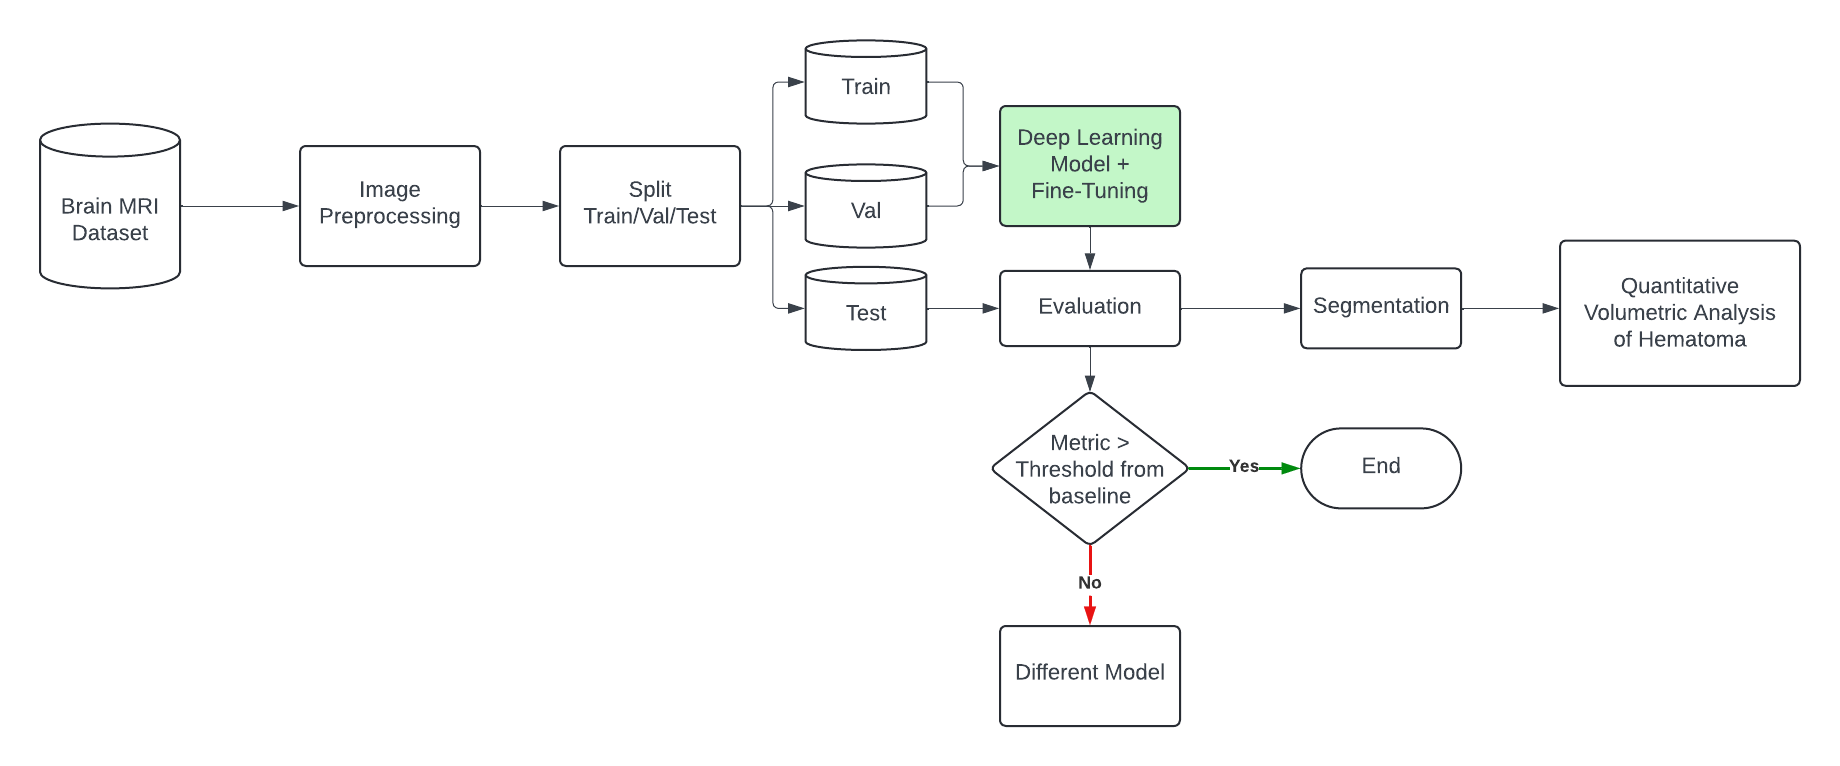
\includegraphics[width = \textwidth]{fig/graphic_workflow (3).png}
\caption{Graphical Workflow}
    \label{fig1}
\end{figure*}
% \begin{figure}[h!]
%     \centering
%     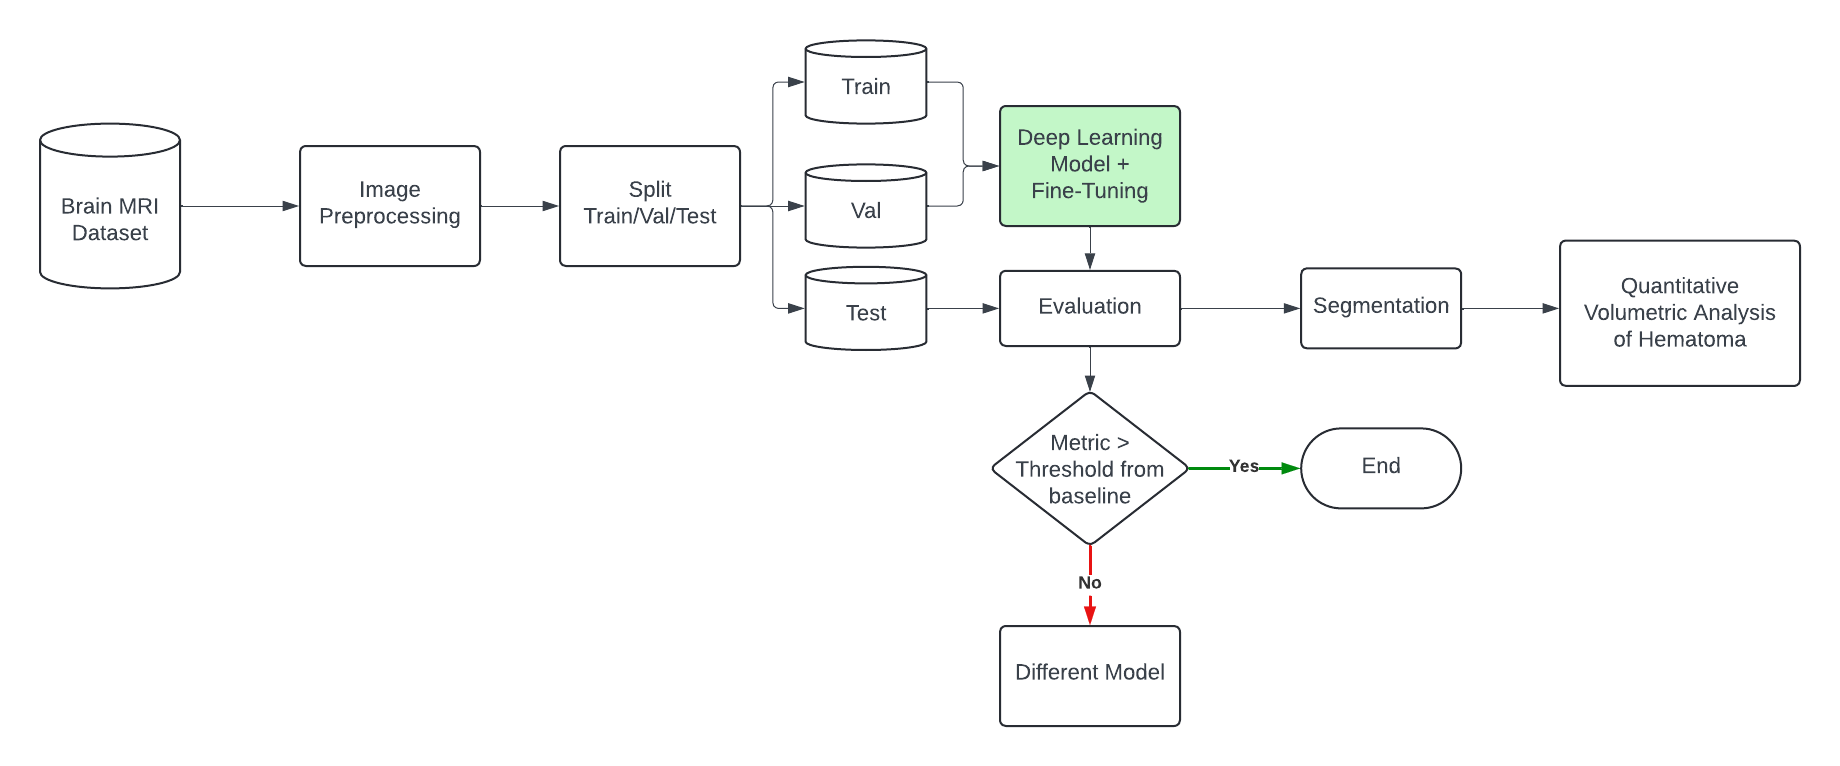
\includegraphics[width = 0.5\textwidth]{fig/graphic_workflow (3).png}
%     \caption{Graphical Workflow}
%     \label{fig:enter-label}
% \end{figure}

% MedSAM introduction https://www.sciencedirect.com/science/article/pii/S1361841523001780#:~:text=Segment%20Anything%20Model%20(SAM)%20is,interactive%20but%20non%2Diterative%20modes.
% fine-tuning based on MedSAM
% fine-tuning using Lora or ConvLora
% baseline: Yangting's model(s)

% lucid chart => segment anything model + generic graphic workflows

\newpage

\bibliographystyle{ieeetr}
\bibliography{ref}
\newpage
\end{document}
